
This part of the section describes how the quench velocity method is applied in a numerical solver. In order to distinguish the quenched zone from the non-quenched one, the superconducting cable is divided into two domains as presented in Fig. \ref{fig:ansys_material_assignment}. The non-quenched part is characterised by nearly zero-resistivity (not zero for the sake of numerical stability) whereas the quenched cable has non-linear resistivity properties of the strand composite as described in (\ref{eqn:strand_resistivity}). The non-linear resistivity is reassigned at each time step as the quench propagates in the model of a numerical solver.

\begin{figure}[H]
\centering
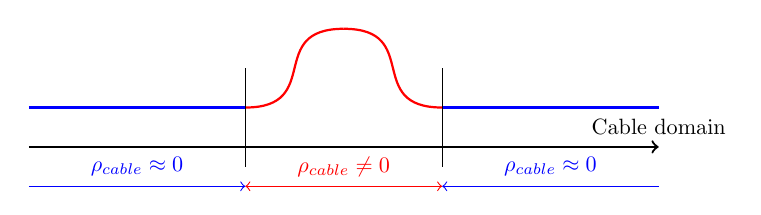
\begin{tikzpicture}[scale = 1]
\draw [thick, ->] (0.0,0.0) -- (8.0,0);
\draw [thick, blue] (0.0,0.5) -- (2.75,0.5);
\draw [thick, blue] (5.25,0.5) -- (8.0,0.5);
\draw [thick, red] (2.75,0.5) .. controls +(0:1cm) and +(180:1cm) .. (4.0,1.5);
\draw [thick, red] (4.0,1.5) .. controls +(0:1cm) and +(180:1cm) .. (5.25,0.5);
\draw [thin] (2.75,-0.25) -- (2.75,1.0);
\draw [thin] (5.25,-0.25) -- (5.25,1.0);
\draw [thin, red, <->] (2.75,-0.5) -- (5.25,-0.5);
\draw [thin, blue, ->] (0.0,-0.5) -- (2.75,-0.5);
\draw [thin, blue, <-] (5.25,-0.5) -- (8.0,-0.5);
\node[scale = 0.8] [color = red] at (4.0,-0.25) {$\rho_\text{cable} \neq 0$};
\node[scale = 0.8] [color = blue] at (1.375,-0.25) {$\rho_\text{cable} \approx 0$};
\node[scale = 0.8] [color = blue] at (6.625,-0.25) {$\rho_\text{cable} \approx 0$};
\node[scale = 0.8] at (8.0,+0.25) {Cable domain};
\end{tikzpicture}
\caption{ANSYS cable domain assignment.}
    \label{fig:ansys_material_assignment}
\end{figure}

The reassignment of material properties should be handled by an external routine which controls the propagation of quench in time. In this case, one should deal with a co-simulation of a numerical solver and a quench velocity estimator. This problem can be handled by means of: 

\begin{itemize}
    \item one-directional exchange of signals,
    \item bi-directional exchange of signals.
\end{itemize}

The one-directional exchange of signals is presented in Fig. \ref{fig:unidirectional_coupling_scheme}. In this case, the numerical solver is provided with a quench front position from the previous communication point $t_{j-1}$ and calculates temperature distribution in the current communication point $t_j$.

\begin{figure}[H]
\centering
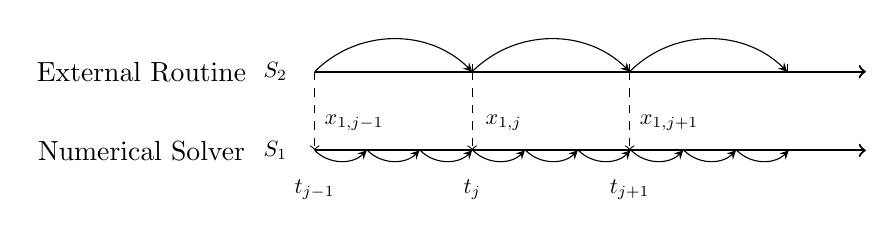
\begin{tikzpicture}[scale = 1]
\draw[thick,->] (0,1) -- (7,1);
\draw (2, 1) -- (2, 1.1);
\draw (4, 1) -- (4, 1.1);
\draw (6, 1) -- (6, 1.1);
\foreach \t in {1,3,5}
\draw [-stealth, bend angle=45, bend left, color = black]  ({\t-1},1) to (\t+1,1);
\draw[thick,->] (0,0) -- (7,0);
\draw (2, 1) -- (2, 1.1);
\draw (4, 1) -- (4, 1.1);
\draw (6, 1) -- (6, 1.1);
\foreach \t in {0.66,1.33,...,6.33}
\draw [-stealth, bend angle=45, bend right]  ({\t-0.66},0) to (\t,0);
\node[scale = 0.8] at (0, -0.5) {$t_{j-1}$};
\node[scale = 0.8] at (2,-0.5) {$t_j$};
\node[scale = 0.8] at (4,-0.5) {$t_{j+1}$};
\draw[dashed, ->] (0,1) -- (0,0);
\draw[dashed, ->] (2,1) -- (2,0);
\draw[dashed, ->] (4,1) -- (4,0);
\node[scale = 0.8] at (-0.5, 0) {$\text{S}_1$};
\node[scale = 0.8] at (-0.5, 1) {$\text{S}_2$};
\node[scale = 0.8] at (0.5, 0.35) {$\text{x}_{1,j-1}$};
\node[scale = 0.8] at (2.4, 0.35) {$\text{x}_{1,j}$};
\node[scale = 0.8] at (4.5, 0.35) {$\text{x}_{1,j+1}$};
\node[color = black] at (-2.2,1.0)	{External Routine};
\node at (-2.2,0)	{Numerical Solver};
\end{tikzpicture}
\caption{Schematic representation of one-directional coupling between a numerical solver and quench velocity estimator.}
\label{fig:unidirectional_coupling_scheme}
\end{figure}

The bi-directional exchange of signals is presented in Fig. \ref{fig:bidirectional_coupling_scheme}. In this case, the external routine is provided with the data from the numerical solver at point $t_j$ to estimate quench velocity at point $t_{j-1}$ up to the point $t_j$. The line which describes the information direction to the external routine is marked in red in Fig.~\ref{fig:bidirectional_coupling_scheme}. 

\begin{figure}[H]
\centering
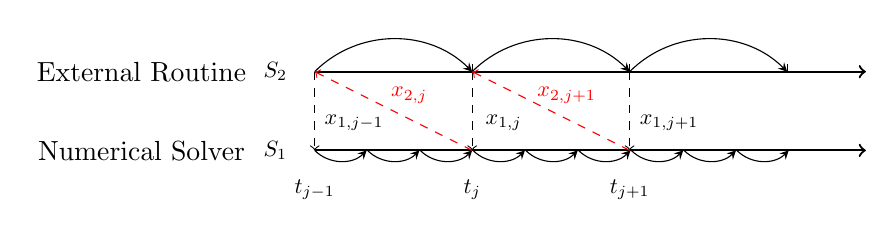
\begin{tikzpicture}[scale = 1]
\draw[thick,->] (0,1) -- (7,1);
\draw (2, 1) -- (2, 1.1);
\draw (4, 1) -- (4, 1.1);
\draw (6, 1) -- (6, 1.1);
\foreach \t in {1,3,5}
\draw [-stealth, bend angle=45, bend left, color = black]  ({\t-1},1) to (\t+1,1);
\draw[thick,->] (0,0) -- (7,0);
\draw (2, 1) -- (2, 1.1);
\draw (4, 1) -- (4, 1.1);
\draw (6, 1) -- (6, 1.1);
\foreach \t in {0.66,1.33,...,6.33}
\draw [-stealth, bend angle=45, bend right]  ({\t-0.66},0) to (\t,0);
\node[scale = 0.8] at (0, -0.5) {$t_{j-1}$};
\node[scale = 0.8] at (2,-0.5) {$t_j$};
\node[scale = 0.8] at (4,-0.5) {$t_{j+1}$};
\draw[dashed, ->] (0,1) -- (0,0);
\draw[dashed, ->] (2,1) -- (2,0);
\draw[dashed, ->] (4,1) -- (4,0);
\draw[dashed, red, ->] (2,0) -- (0,1);
\draw[dashed, red, ->] (4,0) -- (2,1);
\node[scale = 0.8] at (-0.5, 0) {$\text{S}_1$};
\node[scale = 0.8] at (-0.5, 1) {$\text{S}_2$};
\node[scale = 0.8] at (0.5, 0.35) {$\text{x}_{1,j-1}$};
\node[scale = 0.8] at (2.4, 0.35) {$\text{x}_{1,j}$};
\node[scale = 0.8] at (4.5, 0.35) {$\text{x}_{1,j+1}$};
\node[scale = 0.8, red] at (1.2, 0.7) {$\text{x}_{2,j}$};
\node[scale = 0.8, red] at (3.2, 0.7) {$\text{x}_{2,j+1}$};
\node[color = black] at (-2.2,1.0)	{External Routine};
\node at (-2.2,0)	{Numerical Solver};
\end{tikzpicture}
\caption{Schematic representation of bi-directional coupling between a numerical solver and quench velocity estimator.}
\label{fig:bidirectional_coupling_scheme}
\end{figure}

In both cases, the initial quench length is assumed at the beginning of the co-simulation. Between the time steps of the external routine, the numerical solver can handle the problem with an adaptive time step smaller than the communication points $t_j$.

Regardless the type of exchange of signals used, provided that data exchange between an external routine and a numerical solver occurs at communication times $t_j$, the quench velocity algorithm is solved as described in Algorithm~\ref{alg:weak_coupling}.

\begin{algorithm}[H]
  \caption{Weak coupling between a numerical solver and quench velocity estimator.}
  \label{alg:weak_coupling}
  \begin{algorithmic}[1]
    \STATE assume initial quench position $x_{1,j-1}$ 
    \STATE \textbf{for} $j=1,2,...,N$ \textbf{do}
    \STATE \hspace{0.5cm} solve temperature distribution at time $t_j$
    \STATE \hspace{0.5cm} send solver results $x_{2,j}$ to external routine time $t_{j-1}$ (only for bi-directional case)
    \STATE \hspace{0.5cm} estimate new quench position $x_{1,j}$ for a quench front
    \STATE \hspace{0.5cm} assign quench position $x_{1,j}$ to new nodes for solver time  $t_j$
  \end{algorithmic}
\end{algorithm}

As already mentioned, the quench velocity can be: $(i)$ based on available measurements, $(ii)$ calculated numerically, $(iii)$ calculated analytically according to quench velocity equations available in literature. As described in Table~\ref{table:uni_bi_directional_table_explanation}, depending on what quench velocity model is used and which type of geometry is considered, one should choose a one-directional or a bi-directional exchange of signals.

\begin{table}[H]
    \caption{Quench results for analysed time step ranges.} 
    \vspace{-1.em} 
    \fontsize{10}{10}
    \selectfont 
    \renewcommand{\arraystretch}{1.5}
    \begin{center}
        \begin{tabular}{ c | c | c }  
        \hline
         \multirow{2}{*}{$v_\text{quench}$ model} & \multicolumn{2}{c}{geometry type} \\ 
         & one-strand & multi-strand \\
         \hline
        measurements & one-directional & bi-directional \\
        analytical model & one/bi-directional & bi-directional \\
        numerical model & one-directional & bi-directional \\
        \hline 
        \end{tabular}
    \end{center}  
     \label{table:uni_bi_directional_table_explanation} 
 \end{table}

In a one-strand case, if the quench velocity model is based on measurements or a numerical model, the external routine only sends the information to the solver about the quench position in time. Therefore, it is a one-directional exchange of signals. If quench velocity is estimated analytically, the method is either one- or bi-directional. It depends on whether the analytic formula to estimate quench velocity requires additional input data from the solver. In other words, a particular analytic formula may require the value of current or a material property at given temperature which is calculated by a numerical solver. This data would have to be exchanged with an external routine estimating the value of quench velocity. In such a case, a bi-directional exchange of signals is required. In a multi-strand analysis, different winding layers in a magnet interact with one another leading to the transversal heat propagation across the insulation layer. If the temperature outside of a quenched winding also quenches, the external routine has to add a new quench front. Therefore, when a multi-strand model is considered, all quench velocity models are bi-directional.

In this thesis, the quench velocity is estimated numerically.
